\documentclass[tikz,border=4pt]{standalone}
% Shared style for MultiMM figures (white background, logo palette)
\usepackage{tikz,pgfplots,amsmath}
\pgfplotsset{compat=1.16}
\usetikzlibrary{arrows.meta,calc,decorations.pathreplacing,positioning,backgrounds}
\definecolor{indigo}{HTML}{3B37A0}
\definecolor{violet}{HTML}{6A3AA8}
\definecolor{crimson}{HTML}{B5406C}
\definecolor{gold}{HTML}{E9A62C}
\definecolor{golddark}{HTML}{B9791A}
\definecolor{grey}{HTML}{8A8AA0}
\definecolor{lightgrey}{HTML}{E4E4EE}
\tikzset{
  bead/.style={circle,draw=#1!80!black,fill=#1!35,line width=0.5pt,minimum size=9pt,inner sep=0pt},
  bead/.default=indigo,
  lab/.style={font=\small},
}
\pgfplotsset{
  every axis/.append style={
    width=9.5cm,height=6.3cm,axis lines=left,line width=0.5pt,
    grid=major,grid style={draw=lightgrey,line width=0.3pt},
    tick label style={font=\small},label style={font=\normalsize},
    legend style={font=\footnotesize,draw=none,fill=white,fill opacity=0.8,text opacity=1},
    legend cell align=left,
  },
  every axis plot/.append style={line width=1.2pt,smooth},
}

\begin{document}
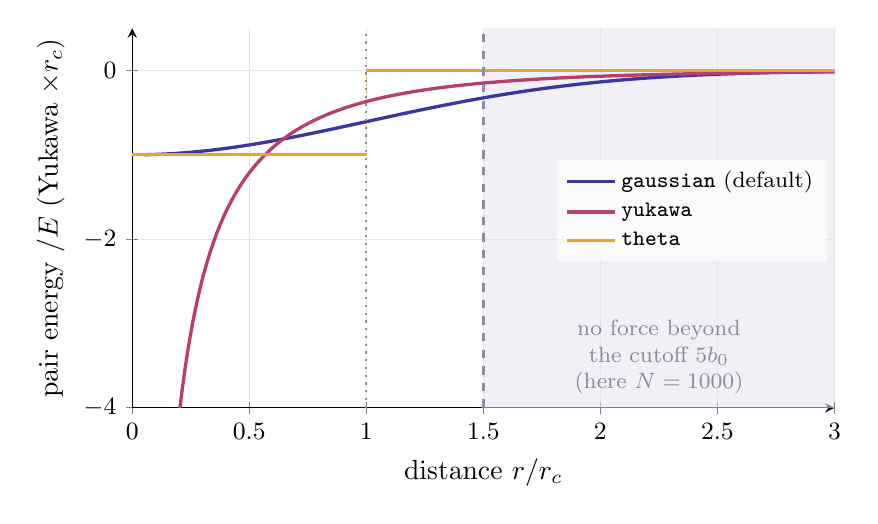
\begin{tikzpicture}
\begin{axis}[width=10.5cm,height=6.4cm,xlabel={distance $r/r_c$},ylabel={pair energy $/E$ (Yukawa $\times r_c$)},
  xmin=0,xmax=3,ymin=-4,ymax=0.5,domain=0.05:3,samples=300,clip=true,restrict y to domain=-4.5:0.5,
  legend style={at={(0.99,0.52)},anchor=east}]
% region beyond the cutoff: the force is switched off
\fill[lightgrey,opacity=0.55] (axis cs:1.5,-4) rectangle (axis cs:3,0.5);
\addplot[indigo] {-exp(-x^2/2)};
\addlegendentry{\texttt{gaussian} (default)}
\addplot[crimson,domain=0.2:3] {-exp(-x)/x};
\addlegendentry{\texttt{yukawa}}
\addlegendimage{gold,line width=1.2pt}
\addlegendentry{\texttt{theta}}
\draw[gold,line width=1.2pt] (axis cs:0,-1)--(axis cs:1,-1);
\draw[gold,line width=1.2pt] (axis cs:1,0)--(axis cs:3,0);
\draw[gold,dotted] (axis cs:1,-1)--(axis cs:1,0);
% r_c: the length scale of the kernels
\draw[grey,dotted,line width=0.8pt] (axis cs:1,-4) -- (axis cs:1,0.5);
\node[font=\footnotesize,grey,anchor=south] at (axis cs:1,0.5) {$r_c$};
% cutoff: pairs farther apart than this feel nothing
\draw[grey,dashed,line width=0.9pt] (axis cs:1.5,-4) -- (axis cs:1.5,0.5);
\node[font=\footnotesize,grey,anchor=south] at (axis cs:1.5,0.5) {cutoff};
\node[font=\footnotesize,grey,align=center] at (axis cs:2.25,-3.4) {no force beyond\\the cutoff $5b_0$\\(here $N=1000$)};
\end{axis}
\end{tikzpicture}
\end{document}
